The \gls{ms} is designed to identify muons and measure their momentum. It is
divided in four sub-detectors, the \gls{mdt}, the \gls{csc}, the \gls{rpc}, and
the \gls{tgc}. The sub-detectors are immersed in a magnetic field generated by
three different toroidal magnets, a barrel toroid covering the $|\eta| < 1.4$
region and two end-caps magnets at $1.6 < |\eta| < 2.7$, which produces a field
almost perpendicular to the muon tracks.

The MDT covers the $|\eta| < 2.7$ region and provides a precise measurement of
the track coordinates in the principal bending direction of the magnetic
field. It uses drift tubes to reconstruct the muon trajectory and the drift time
of the ionized charges is used to determine the minimum distance between the
wire and the muon. The CSC covers the $2.0 < |\eta| < 2.7$ region and is a
multi-wire proportional chamber with cathodes segmented in strips, one
perpendicular to the anode wire, providing the precision coordinate, and the
other parallel to it (giving the transverse coordinate).


The RPC and the TGC cover the $|\eta| < 1.05$ and $1.05 < |\eta| < 2.7$ regions
respectively. They contribute to the Level 1 trigger providing bunch crossing
identification, it allows to select high and low $\pt$ tracks and measure the
muon coordinate in the direction orthogonal to that determined by MDT and CSC\@.

\begin{figure}[!h]
  \centering
    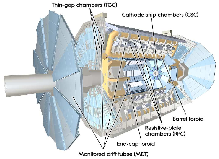
\includegraphics[width=.7\linewidth]{muon_spectro}
    \caption{Cut-away view of the ATLAS muon spectrometer~\cite{ATLASPaper}.}
    \label{fig:muon_spectro}
\end{figure}
%%% Local Variables:
%%% mode: latex
%%% TeX-master: "../search_for_DM_LED_with_ATLAS"
%%% End:
